\documentclass[11pt,leqno]{article}
\usepackage[T1]{fontenc}
\usepackage[polish]{babel}
\usepackage[utf8]{inputenc}
\usepackage{a4wide}
\usepackage{amsmath}
\usepackage{amsfonts}
\usepackage{graphicx}
\usepackage{algpseudocode}
\usepackage{algorithm}

\newcommand{\dvar}[1]{\,\mathrm{d}#1}

\title{
  \textbf{Pracownia 3 z analizy numerycznej}\\
  \textit{Zadanie 8}
}
\author{Łukasz Hanuszczak}
\date{Wrocław, \today}

\begin{document}
\maketitle


\section{Wstęp}

\subsection{Całki wielokrotne}
Całka podwójna to całka po dwóch zmiennych pewnej funkcji $f: \mathbb{R} \times \mathbb{R} \to \mathbb{R}$:
\[
  \int_a^b \int_c^d f(x, y) \,\mathrm{d}y \,\mathrm{d}x
\]

Interpretacja geometryczna całki podwójnej jest analogiczna do całki pojedyńczej: jeżeli $\int_a^b g(x) \,\mathrm{d}x$ jest polem pod wykresem funkcji $g$ na przedziale $[a, b]$ to $\int_a^b \int_c^d f(x, y) \,\mathrm{d}y \,\mathrm{d}x$ jest objętością zawartą między płaszczyzną $z = 0$ a powierzchnią $z = f(x, y)$ na prostokącie $[a, c] \times [b, d]$. Podobnie jak zwykłe całki pojedyńcze, obliczanie całek podwójnych ma liczne zastosowania praktycznie.

Oczywiście tak sformułowaną definicję łatwo rozszerzyć na całki $n$-krotne działające na $n$-wymiarowych przestrzeniach. Jak się okaże, obliczanie całek $n$-krotnych wcale nie jest dużo trudniejszym zadaniem (pomijając rosnący koszt obliczeniowy) i zaproponowane rozwiązanie bardzo łatwo daje się rozszerzać.


\subsection{Ogólny sposób obliczania}
Intuicyjnie, wystarczy sprowadzić całkę podwójną do całki pojedynczej (bardziej ogólnie: całkę $n$ zmiennych do całki $(n - 1)$ zmiennych) i dalej stosować poznane już metody.
\[
  \int_a^b \int_c^d f(x, y) \,\mathrm{d}y \,\mathrm{d}x
=
  \int_a^b \left( \int_c^d f(x, y) \,\mathrm{d}y \right) \,\mathrm{d}x
=
  \int_a^b g(x) \,\mathrm{d}x
\]
gdzie
\[
  g(x) = \int_c^d f(x, y) \,\mathrm{d}y
\]
Przykładowo, symboliczna droga obliczenia całki z treści zadania mogłaby być następująca. Niech:
\[
  V = \int_0^1 \int_0^1 \frac{\mathrm{d}y \,\mathrm{d}x}{x^2 + y^2 + 1}
\]
Podstawiając kolejno:
\[
  g(x)
=
  \int_0^1 \frac{\mathrm{d}y}{x^2 + y^2 + 1}
=
  \int_0^1 \frac{\mathrm{d}y}{x^2 + t^2}
=
  \left[ \frac{\arctan \frac{x}{t}}{t} \right]_0^1
=
  \left[ \frac{\arctan \frac{x}{\sqrt{y^2 + 1}}}{\sqrt{y^2 + 1}} \right]_0^1
=
\]
\[
=
  \frac{\arctan \frac{x}{\sqrt{1^2 + 1}}}{\sqrt{1^2 + 1}}
  -
  \frac{\arctan \frac{x}{\sqrt{0^2 + 1}}}{\sqrt{0^2 + 1}}   
=
  \frac{\arctan \frac{x}{\sqrt{2}}}{\sqrt{2}} - \arctan x   
\]
W ten sposób zadanie zostało sprowadzone do obliczenia zwykłej, pojedynczej całki:
\[
  V
=
  \int_0^1 g(x) \,\mathrm{d}x
=
  \int_0^1
    \frac{\arctan \frac{x}{\sqrt{2}}}{\sqrt{2}} - \arctan x
  \,\mathrm{d}x
\]

W przypadku obliczeń numerycznych rzecz jest niewiele trudniejsza. Dla wielokrotnych całek wystarczy zastosować wybraną przez siebie metodę (albo wybrać podejście hybrydowe lub adaptacyjne) wielokrotnie. Mając zatem gotowe rozwiązania dla obliczania zwykłych funkcji bez problemu można bez zbędnego wysiłku szybko rozszerzyć je na całki dwu-, trzy- a nawet $n$-krotne.

W dalszej części opisano więc kilka standardowych metod obliczania całek i zaprezentowano wyniki ich działania na całkach dwukrotnych.



\section{Metody obliczania}


\subsection{Kwadratury Newtona-Coatesa}
Kwadratury Newtona-Coatsa to kwadratury interpolacyjne (a więc takie, które wykorzystują wielomiany interpolacyjne do przybliżania wartości funkcji) z równoodległymi węzłami. W dalszym tekście przedstawione zostanie tylko dwóch najprostszych reprezentantów tej klasy kwaratur: wzór trapezów oraz metoda Simpsona.

\subsubsection{Złożony wzór trapezów}
Wzór trapezów to nic innego jak oszacowanie wartości całki oznaczonej na przedziale $[a; b]$ jako pola trapezu o podstawach długości $f(a)$ i $f(b)$:
\[
  \int_a^b f(x) \dvar{x} \approx \frac{f(a) + f(b)}{2}
\]

Oczywiście szacowana w ten sposób wartość całki z reguły jest bardzo niedokładna. Dlatego zarówno w przypadku wzoru trapezów jak i każdej innej kwadratury stosuje się tak zwane ,,wzory złożone''. Polegają one na podziale przedziału $[a; b]$ na $k + 1$ podprzedziałów $[a; t_1], [t_1; t_2], \dots, [t_k, b]$ i zastosowania danego wzoru na mniejszym przedziale, minimalizując w ten sposób wartości błędu. Najczęściej punkty $t_1, \dots, t_k$ są dobierane jako równoodległe. Ostatecznie złożony wzór trapezów prezentuje się następująco:
\[
  \int_a^b f(x) \dvar(x)
\approx
  \frac{b - a}{k} \sum_{i = 0}^{k} {}^{''} f(a + i \frac{b - a}{k})
\]


\subsubsection{Metoda Simpsona}
Kolejnym w miarę prostym sposobem obliczania całek numerycznych jest metoda Simpsona. Analogicznie do wzoru trapezów, metoda stara się przybliżać daną funkcję na przedziałach za pomocą funkcji dużo prostszych. O ile w metodzie trapezów wykorzystywane były po prostu funkcje liniowe (odcinki), tak tutaj są to odpowiednio funkcje kwadratowe.

Mając dane 3 równoodległe punkty, $x_0, x_1, x_2$ wartość całki funkcji $f$ na przedziale $[x_0; x_2]$ można przybliżyć za pomocą wzoru:
\[
  \int_{x_0}^{x_2} f(x) \,\mathrm{d}x
\approx
  \frac{h}{3} \left( f(x_0) + 4f(x_1) + f(x_2) \right)
\]

Stąd nietrudno już dojść do złożonej wersji tego wzoru:
\[
  \int_{a}^{b} f(x) \,\mathrm{d}x
\approx
  \frac{b - a}{3} \left(
      f(x_0)
    +
      4 \sum_{i = 1}^{\frac{k}{2} - 1} f(x_{2i - 1})
    +
      2 \sum_{i = 1}^{\frac{k - 1}{2}} f(x_{2i}) + y
  \right)
\]

\subsection{Metoda Romberga}
Metoda Romberga jest swego rodzaju ,,ulepszeniem'' metody trapezów. Wprowadzoną modyfikacją jest zastosowanie tzw. ekstrapolacji Richardsona, czyli techniki poprawiającej zbieżność ciągów.

Do znalezienia przybliżonej wartości całki funkcji $f$ na przedziale $[a; b]$ konstruuje się trójkątną tablicę według poniższych zależności rekurencyjnych:
\[
  R(0, 0) = (b - a)\frac{f(a) + f(b)}{2}
\]
\[
  R(n, 0) = \frac{R(n - 1, 0)}{2} + h_n \sum_{k = 1}^{2^{n - 1}}
    f(a + (2k - 1)h_n)
\]
\[
  R(n, m) = R(n, m - 1) + \frac{1}{4^m - 1}
  \left(
    R(n, m - 1) - R(n - 1, m - 1)
  \right)
\]
\[
  h_n = \frac{b - a}{2^n}
\]
Stablicowane wartości $R(n, m)$ odpowiadają zastosowaniu $m$-tej kwadratury Newtona-Coatesa przy wykorzystaniu wielomianu interpolacyjnego $n$-tego stopnia. Mimo szybko rosnącej złożoności obliczania kolejnych wierszy, metoda Romberga daje z reguły dobre przybliżenia całki już dla niewielkich wartości $n$ i jest bardzo często wykorzystywana w praktyce.


\subsection{Kwadratury Gaussa-Legendre'a}
Kwadratury Gaussa to klasa kwadratur interpolacyjnych oferująca najlpszy rząd wynąszący $2n + 2$. O ile kwadratury Newtona-Coatesa wykorzystywały wielomiany interpolacyjne i równoodległe węzły, tak kwadratury Gaussa wykorzystują wielomiany ortogonalne. I tak dla funkcji wagowej $p(x) = 1$ (czyli tej najczęściej stosowanej) używają tzw. wielomianów Legendre'a i ich pierwiastków. Brak niestety na nie ogólnych wzorów, a obliczanie ich samodzielnie mogłoby okazać się zbyt pracochłonne. Dlatego na ogół wykorzystuje się gotowe tablice, dostępne między innymi w Internecie. Dzięki temu otrzymuje się metodę banalną w implementacji, która nawet dla niewielkich wartości $n$ będzie dawała bardzo satysfakcjonujące wyniki. Aby pokazać wyższość tej metody w poniższej analizie będzie uwzględniona kwadratura Gaussa-Legendre'a wykorzystująca zaledwie 5 węzłów na danym przedziale.


\section{Analiza}

Przybliżone wartości całek z którymi porównywane były wyniki programu zostały obliczone przy pomocy portalu \textit{Wolfram Alpha} i oprogramowania \textit{MATLAB}. W przypadku niektórych testowanych funkcji konieczne było wprowadzenie modyfikacji, która pozwalałaby uniknąć dzielenia przez zero. Dla uproszczenia, w miejscu gdzie funkcja nie osiągała żadnej wartości przyjęto $0$. Poniższe wykresy prezentują zależność wartości funkcji błędu od ilości podprzedziałów (wierszy w przypadku tablicy Romberga). 

\subsection{Funkcja $f(x, y) = 1 / (x^2 + y^2 + 1)$}
Treść zadania sugeruje przetestowanie metod na stosunkowo prostej i gładkiej funkcji.
\[
  \int_{0}^{1} \int_{0}^{1} \frac{1}{x^2 + y^2 + 1} \dvar{y} \dvar{x}
\approx
  0.639510351870311001962693085427323679
\]

\begin{center}
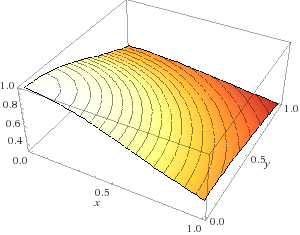
\includegraphics[scale=0.65,natwidth=640,natheight=480]{gfx/test1g.png}
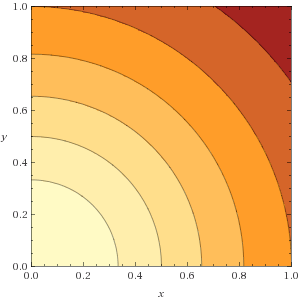
\includegraphics[scale=0.65,natwidth=640,natheight=480]{gfx/test1p.png}\\
\end{center}

Zgodnie z intuicją, obydwie testowane kwadratury Newtona-Coatsa zostają zdeklasowane przez metodę Romberga i kwadraturę Gaussa. Oczywiście przyrównywanie tych dwóch ostatnich do siebie na jednym wykresie nie ma większego sensu ze względu na ich zupełnie różne złożoności obliczeniowe. Obydwie metody zostały naniesione na jeden wykres tylko ze względu na oszczędność miejsca.
 
Warto również odnotować, że dla $k = 12$ metoda Romberga osiąga maksymalną możliwą dokładność w arytmetyce podwójnej precyzji (a dla $k \in \{9, 10, 11\}$ błąd wynosi mniej niż $10^{-16}$) po czym zaczyna wzrastać. Jest to oczywiście spowodowane rosnącą liczbą wykonywanych operacji arytmetycznych, co wiąże się z szybszą kumulacją błędów.

Ciekawie również wypada porównanie metody Simpsona i Trapezów. Z wykresu można wywnioskować, że ta pierwsza zachowuje się dużo mniej stabilnie dając dużo gorsze wyniki dla nieparzystych wartości $k$.

\begin{center}
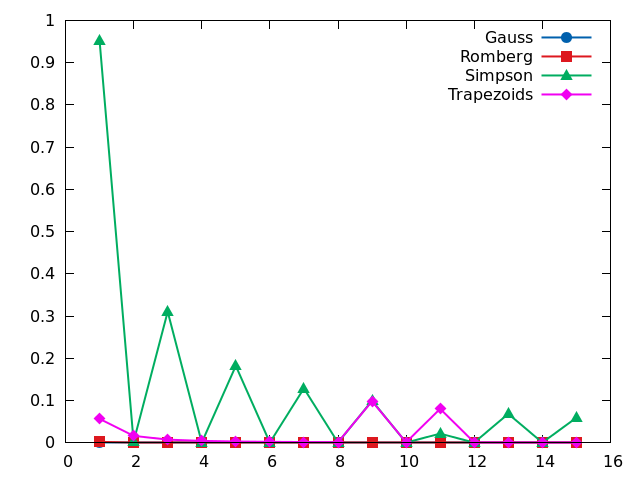
\includegraphics[scale=0.65,natwidth=640,natheight=480]{plot/test1_15e.png}\\
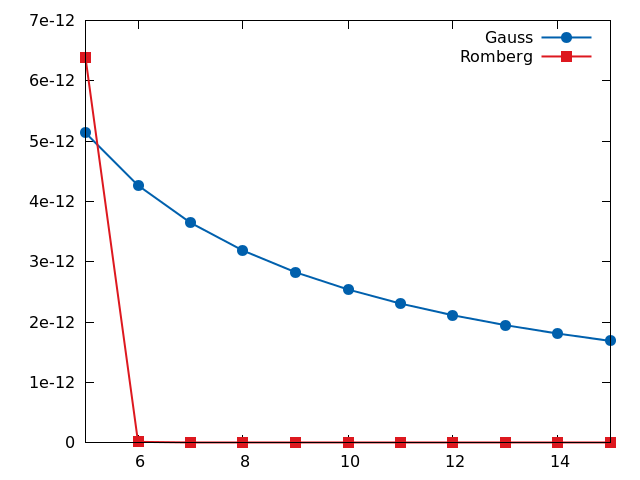
\includegraphics[scale=0.65,natwidth=640,natheight=480]{plot/test1_15ezoom.png}\\
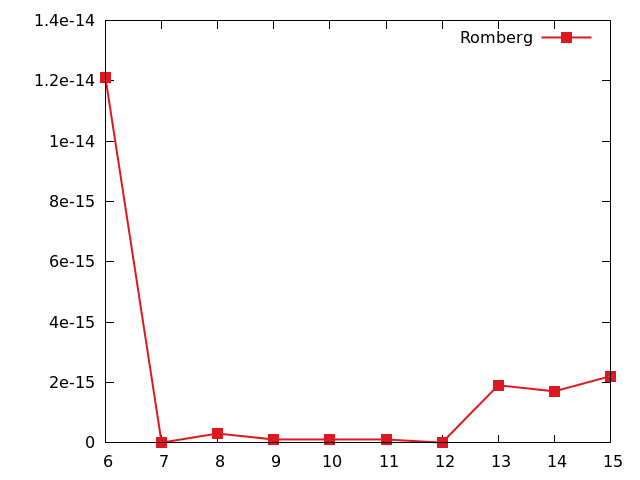
\includegraphics[scale=0.65,natwidth=640,natheight=480]{plot/test1_r15ezoom.png}
\end{center}


\subsection{Funkcja $f(x, y) = (x - 1) / ((1 - xy) \ln xy)$}

\[
  \int_{0}^{1} \int_{0}^{1} \frac{x - 1}{(1 - xy) \ln xy} \dvar{y} \dvar{x}
\approx
  0.5772079363088510328694269
\]

\begin{center}
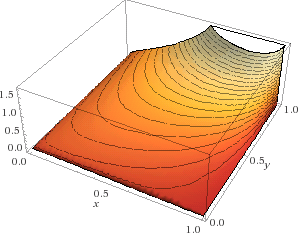
\includegraphics[scale=0.65,natwidth=640,natheight=480]{gfx/testa1g.png}
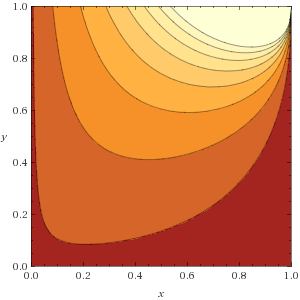
\includegraphics[scale=0.65,natwidth=640,natheight=480]{gfx/testa1p.png}\\
\end{center}

Patrząc na powyższy wykres funkcja nie wygląda nadzwyczajnie. Mimo to powoduje bardzo dziwne zachowanie metody Gaussa. Metoda zamiast polepszać swoją dokładność, wręcz przeciwnie, tylko oddala się od dokładnego wyniku. Zjawisko to nie występuje w przypadku innych kwadratur, które radzą sobie całkiem dobrze. Stanowi to ewenement spośród testowanych funkcji i jest jedynym testem w którym metoda Gaussa ,,nie podołała''.

Patrząc tylko na pozostałe metody, ponownie można zauważyć pogarszanie się wyników metody Simpsona dla nieparzystych wartości $k$, oraz niespodziewany wzrost wartości błędu złożonego wzoru trapezów dla $k = 9$ i $k = 10$.

Z kolei metoda Romberga, mimo wyraźnej przewagi nad konkurentkami nie sprawuje się tak dobrze jak poprzednio. Dokładność owszem rośnie, ale dość wolno biorąc pod uwagę jej złożoność i to jak wypada w pozostałych testach. I tak dla $k = 14$ i bardzo długiego czasu potrzebnego do wyznaczenia wartości, metoda daje zaledwie 5 cyfr dokładnych po przecinku.

\begin{center}
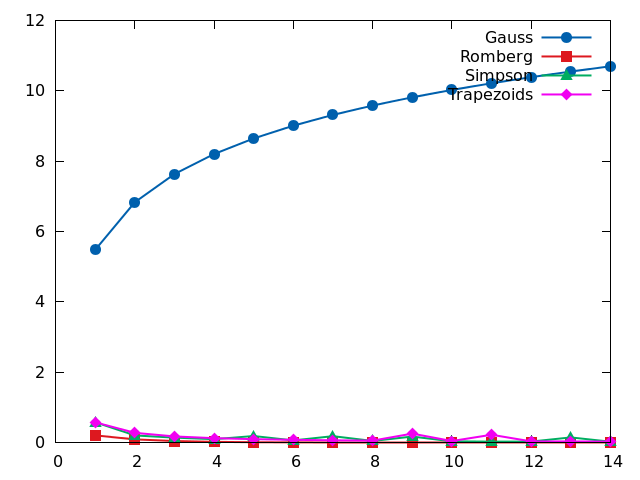
\includegraphics[scale=0.65,natwidth=640,natheight=480]{plot/testa1_14e.png}\\
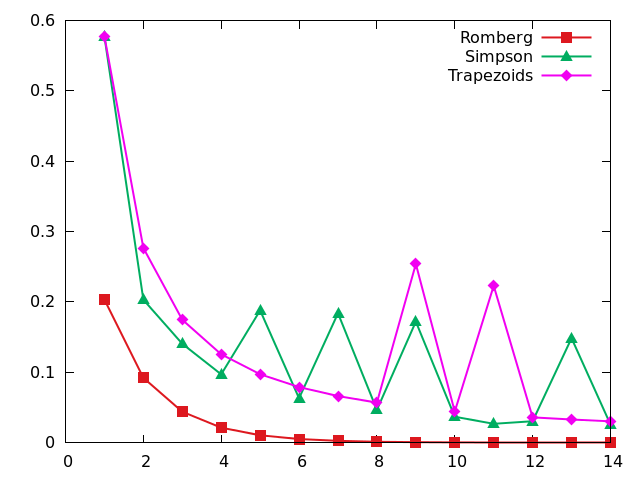
\includegraphics[scale=0.65,natwidth=640,natheight=480]{plot/testa1_14ezoom.png}
\end{center}



\subsection{Funkcja $f(x) = 1 / \sqrt{1 + x^2 + y^2}$}
\begin{center}
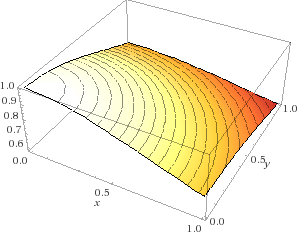
\includegraphics[scale=0.65,natwidth=640,natheight=480]{gfx/testa3g.png}
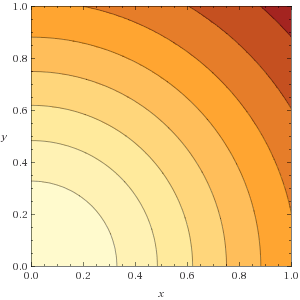
\includegraphics[scale=0.65,natwidth=640,natheight=480]{gfx/testa3p.png}\\
\end{center}

Funkcja ta w zasadzie jest spierwiastkowaną werjsą pierwszej funkcji testowej (z treści zadania). Z tego powodu wyniki wykresów błędów są niemal identyczne z tymi już prezentowanymi wcześniej.

\begin{center}
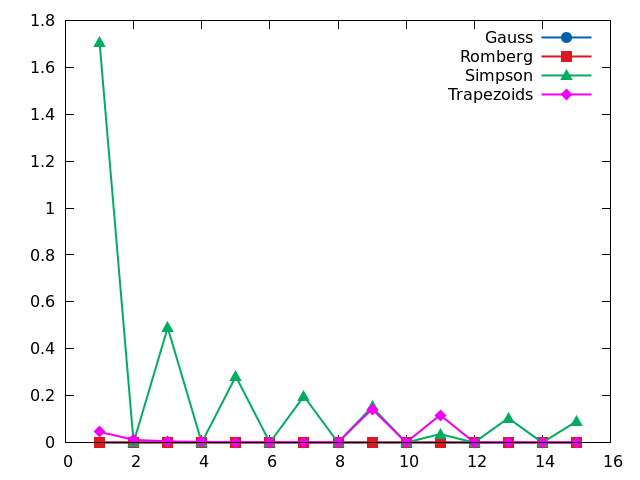
\includegraphics[scale=0.65,natwidth=640,natheight=480]{plot/testa3_15e.png}
\end{center}


\subsection{Funkcja $f(x) = 1 / (1 - xy) $}
\[
  \int_{0}^{1} \int_{0}^{1} \frac{1}{1 - xy} \dvar{y} \dvar{x}
\approx
  1.644940990771051492203014
\]
\begin{center}
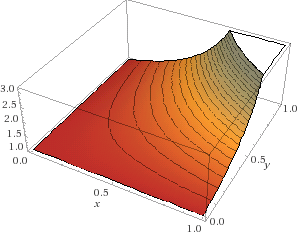
\includegraphics[scale=0.65,natwidth=640,natheight=480]{gfx/testa4g.png}
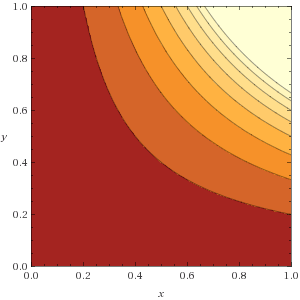
\includegraphics[scale=0.65,natwidth=640,natheight=480]{gfx/testa4p.png}\\
\end{center}

Wyniki tylko potwierdzają wcześniejsze obserwacje. Metoda Simpsona po raz kolejny zachowuje się niestabilnie i nawet dla parzystych wartości $k$ jest niewiele lepsza od złożonego wzoru trapezów. Tak jak wspomniano poprzednio, porównywanie ze sobą metod Gaussa i Romberga nie ma większego sensu ze względu na dość szybko rosnący czas wykonania tej drugiej. Warto jednak odnotować, że dla $k < 8$, czyli do momentu kiedy metoda Romberga zaczyna zauważalnie spowalniać wyniki otrzymywane przez kwadraturę Gaussa są lepsze i uzyskane dużo mniejszym kosztem.

\begin{center}
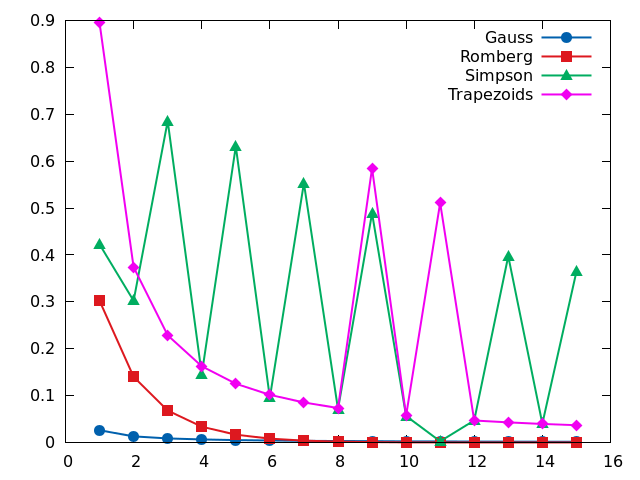
\includegraphics[scale=0.55,natwidth=640,natheight=480]{plot/testa4_15e.png}\\
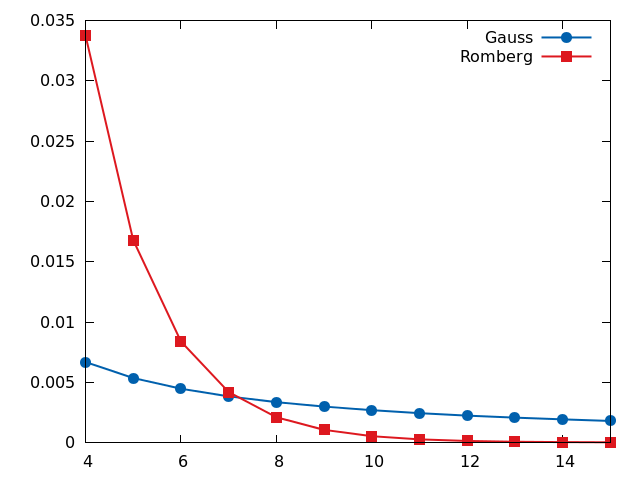
\includegraphics[scale=0.55,natwidth=640,natheight=480]{plot/testa4_15ezoom.png}
\end{center}


\subsection{Inne}
\[
  f(x, y)
=
  \frac{\pi^2 (1 + x) \sin(\pi (1 + x))}{(1 - x)(3 + x)}
  \frac{\pi^2 (1 + y) \sin(\pi (1 + y))}{(1 - y)(3 + y)}
\]

\[
  \int_{-1}^{1} \int_{-1}^{1} f(x, y) \dvar{y} \dvar{x}
\approx
  216.885736591036128289135904407106432210
\]

Jak widać, funkcja ta jest dużo bardziej złożona od wszystkich powyższych. Dzięki swojemu dość przypadkowemu wizerunkowi daje ciekawy materiał porównawczy.

Najbardziej w oczy rzuca się bezkonkurencyjny wynik kwadratury Gaussa, który deklasuje pozostałe metody zarówno pod względem szybkości zbieżności jak i czasu działania. Wykonując (względnie) niewiele więcej operacji od metody Simpsona daje nawet dla jednego przedziału rewelacyjną dokładność.
Zawodzi natomiast metoda Romberga. Nie dość, że czas jej wykonania dla $k = 15$ liczony jest w minutach to i tak ledwo osiąga wynik, który kwadratura Gaussa zwraca natychmiastowo.

Jeżeli chodzi o kwadratury Newtona-Coatesa widać bardzo dużą niestabilność, tym razem także i w przypadku wzoru trapezów. W obydwu wypadkach wyniki przez moment się polepszają by za chwilę znów oddalić się od oczekiwanego rezultatu. Warto również zwrócić uwagę na skalę tego zjawiska - błąd na pierwszym wykresie jest przecież liczony w setkach.

\begin{center}
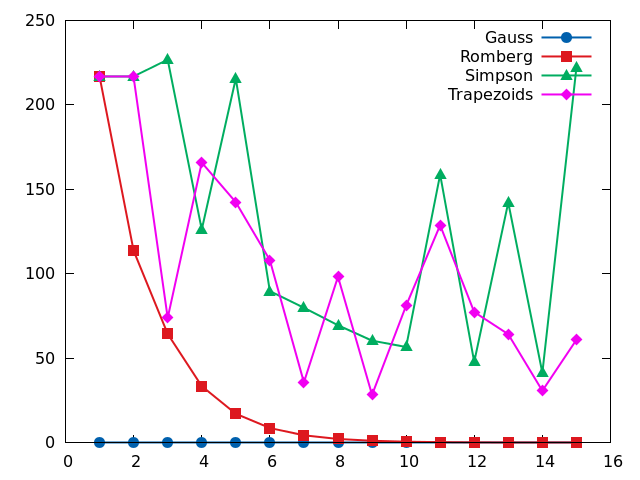
\includegraphics[scale=0.65,natwidth=640,natheight=480]{plot/test3_15e.png}\\
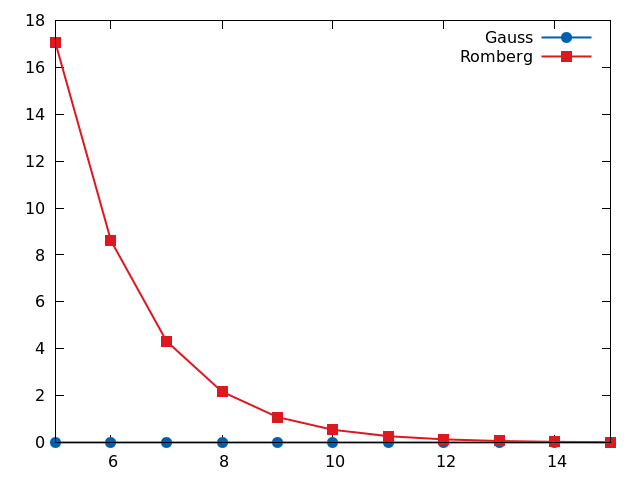
\includegraphics[scale=0.65,natwidth=640,natheight=480]{plot/test3_15ezoom.png}\\
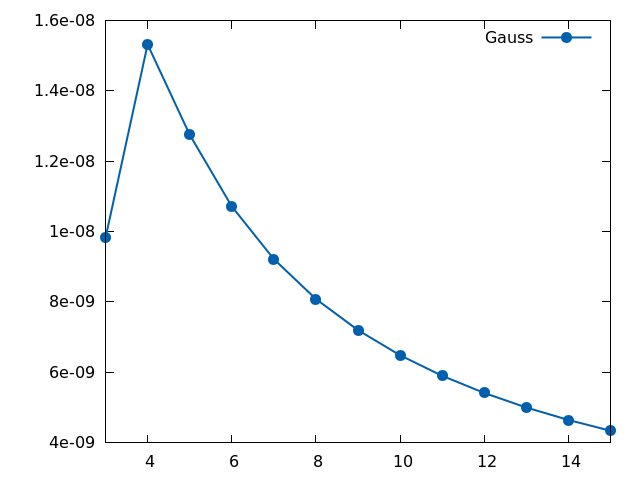
\includegraphics[scale=0.65,natwidth=640,natheight=480]{plot/test3_g15ezoom.png}
\end{center}


\section{Podsumowanie}
Na podstawie powyższych analiz bezapelacyjnie kwadratura Gaussa jest zdecydowanie najlepszą metodą obliczania całek (w tym podwójnych), nawet z użyciem tak niewielkiej ilości węzłów. Jest wystarczająco szybka zarówno pod względem wydajnościowym jak i ,,zbieżnościowym''. Mimo skomplikowanej matematycznej maszynerii za nią stojącej, dzięki możliwości stablicowania wag i pierwiastków wielomianów Legendre'a, jest w implementacji prostsza niż choćby metoda Simpsona. Oczywiście, nie ma rzeczy idealnych i zawsze istnieją przypadki gdy inne podejście okaże się lepszym. Świadczyć o tym może choćby drugi przypadek testowy. Dlatego warto zastanowić się nad rozwiązaniem hybrydowym lub jakimś wariantem metod adaptacyjnych, które mogą naprawić ,,patologiczne'' przypadki.


\begin{thebibliography}{99}
\bibitem{Kincaid} David Kincaid, Werd Cheney, Analiza Numeryczna (2006)
\bibitem{Jankowscy} Janina i Michał Jankowscy, Przegląd metod i algorytmów numerycznych (1981)
\bibitem{WikiDIntegral} http://en.wikipedia.org/wiki/Double\_integral
\bibitem{Holoborodko} Pavel Holoborodko, http://www.holoborodko.com/pavel/numerical-methods/numerical-integration/
\end{thebibliography}

\end{document}